\documentclass{article}

\usepackage[utf8]{inputenc}
\usepackage{lmodern}
\usepackage{ngerman}
\usepackage{graphicx}

\begin{document}


\textbf{Aufgabe 1}
\textbf{a) Wahrscheinlichkeit zwischen $\frac{1}{2}$ und $\frac{1}{3}$} \\

\[
P\left(A\right) - P\left(B\right)
\]
\[
P\left(x \le \frac{1}{2}\right) - P\left(x \le \frac{1}{3}\right)
\]

Bei einer Gleichverteilung ist die summierte Wahrscheinlichkeit gleich dem Grenzwert.

\[
= \frac{1}{2} - \frac{1}{3} = \frac{3}{6} - \frac{2}{6} = \frac{1}{6}
\]
 \\

\textbf{b) Wahrscheinlichkeit von $\frac{1}{2}$} \\

\[
P(A) = \frac{k}{n} = \frac{G\"unstige F\"alle} {M\"ogliche F\"alle}
\]

Wir betrachten eine Gleichverteilung im Intervall $[0,1]$ reeller Zahlen.

G\"unstiger Fall, Wert $\frac{1}{2}: 1$ \\
M\"ogliche F\"alle: unendlich
\[
\frac{1}{\infty} = 0
\]
\\

\textbf{c) Wahrscheinlichkeit von $\frac{1}{2}$ in einem Zufallsgenerator auf dem Computer} \\

Um die Wahrscheinlichkeit eines exakten Wertes in einem Zufallsgenerator auf einem
Computer zu bestimmen, pr\"ufen wir, ob diese Zahl auch als bin\"are Gleitkommazahl darstellbar ist.
Wir betrachten den Wert $\frac{1}{2}$, zun\"achst die erste Bin\"arstelle:

\[
 2^{-1} = 1,
\]

fuer alle weiteren Bin\"arstellen gilt

\[
2^{-2} = 2^{-3} = ... = 2^{-23} = 0
\]

Gehen wir von einer theoretischen perfekten Gleichverteilung auf einem Computer aus, 
so hat man einen g\"unstigen Fall zu $2^{23}$ m\"oglichen F\"allen.
Die Wahrscheinlichkeit $\frac{1}{2}$ zu treffen ist somit

\[
P\left(\frac{1}{2}\right) = \frac{1}{2^{23}} =\frac{1}{8388608}
\]


Nutzt man nun die Zufallsgeneratoren von Numpy oder ROOT, so sollte unter rund $10000000$ Ereignissen
 der gesuchte exakte Wert sein. Wir haben dies mit der doppelten Anzahl von Zufallszahlen 
und der Verwendung von numpy.random und ROOT.TRandom durchlaufen lassen. 
Das Ergebnis ist in Bild 1 zu sehen.
 \\
\begin{figure}[htbp]
	\centering
	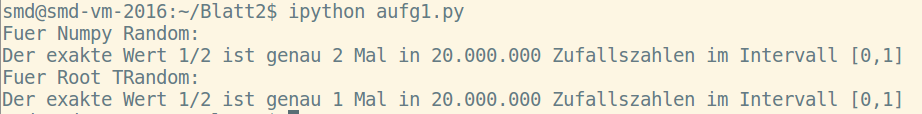
\includegraphics[width=0.7\textwidth]{Gleichvert1zu2.png}
	\caption{Haeufigkeit Zufallszahlen}
\end{figure}
 \\

\textbf{d) Wahrscheinlichkeit von $\frac{2}{3}$ in einem Zufallsgenerator auf dem Computer} \\

Der Wert $\frac{2}{3}$ l\"asst sich nicht exakt als bin\"are Gleitkommazahl darstellen,
somit ist es einem Zufallsgenerator mit binaeren Gleitkommazahlen nicht m\"oglich,
den Wert exakt darzustellen. Die Berechnung ist in Bild 2 zu sehen. 
Die Addition von jedem ungeraden Exponenten n\"ahert den exakten Wert an, 
jeder gerade Exponent wird \"ubersprungen, da sonst die $\frac{2}{3}$  \"uberschritten werden.

\\

\begin{figure}[htbp]
	\centering
	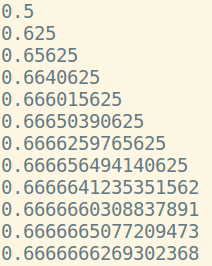
\includegraphics[width=0.4\textwidth]{Binaer2zu3.png}
	\caption{Berechnung im Binaersystem}
\end{figure}




\end{document}